\documentclass[10pt,a4paper]{article}

\usepackage[utf8]{inputenc}
\usepackage[T1]{fontenc}
\usepackage[brazil]{babel}
\usepackage[a4paper,margin=1cm]{geometry}
\usepackage{multicol}
\usepackage{graphicx}
\usepackage{booktabs}
\usepackage{array}
\usepackage{listings}
\usepackage{xcolor}
\usepackage{microtype}
\usepackage{fancyhdr}

\setlength{\parindent}{0pt}
\setlength{\parskip}{3pt}
\setlength{\columnsep}{0.7cm}
\pagestyle{fancy}
\fancyhf{}
\fancyfoot[C]{Grupo 11 --- TP1 OpenMP \quad | \quad Página \thepage}
\renewcommand{\headrulewidth}{0pt}

\definecolor{codegray}{rgb}{0.96,0.96,0.96}
\lstset{
  language=C,
  basicstyle=\ttfamily\scriptsize,
  numbers=left,
  numberstyle=\tiny\color{gray},
  stepnumber=1,
  numbersep=7pt,
  backgroundcolor=\color{codegray},
  frame=single,
  breaklines=true,
  showstringspaces=false,
  tabsize=4,
  keywordstyle=\color{blue!70!black},
  commentstyle=\color{green!40!black},
  stringstyle=\color{red!60!black}
}

\newcommand{\secao}[1]{\vspace{2pt}\textbf{\large #1}\par}

\begin{document}

\begin{center}
  {\Large\textbf{Busca paralela de texto com OpenMP}}\\[-1pt]
  Computação Paralela --- TP1 --- Grupo 11\\
  Integrantes: \rule{10cm}{0.4pt}
\end{center}

\begin{multicols}{2}

\secao{1. Problema}

A aplicação busca uma palavra em vários arquivos TXT e informa as ocorrências
por arquivo e o total. A busca é literal, diferencia maiúsculas de minúsculas e
não conta ocorrências sobrepostas. O tempo inclui abertura, leitura, busca e
fechamento dos arquivos.

Há potencial de paralelização porque cada arquivo pode ser pesquisado
independentemente. Os principais limites são o acesso ao sistema de arquivos e
o desbalanceamento provocado por arquivos de tamanhos diferentes.

\secao{2. Implementação OpenMP}

A versão sequencial percorre os arquivos em ordem. A versão paralela aplica:

\begin{center}
\small\texttt{parallel for schedule(runtime) reduction(+:total)}
\end{center}

\texttt{parallel for} distribui os arquivos entre as threads.
\texttt{reduction} soma os resultados sem condição de corrida.
\texttt{schedule(runtime)} permite comparar os escalonadores \texttt{static},
\texttt{dynamic} e \texttt{guided} sem recompilar. Cada iteração escreve em uma
posição exclusiva do vetor de resultados, dispensando região crítica.

\secao{3. Metodologia}

As medições foram feitas no nodo \texttt{atlantica07} do LAD, com dois
processadores Xeon E5520, oito núcleos físicos e 16 threads lógicas. O código
foi compilado com GCC 9.4.0, \texttt{-O2} e \texttt{-fopenmp}. Foram usados
\texttt{OMP\_PROC\_BIND=spread} e \texttt{OMP\_PLACES=cores}.

Cada configuração teve aquecimento e 15 execuções; a mediana foi usada por ser
menos sensível a variações. Na escalabilidade forte foram mantidos 1.024
arquivos e 105,8 MB. Na fraca, foram mantidos 64 arquivos e 6,61 MB por thread.

Os arquivos originais eram pequenos demais para medições estáveis. Por isso,
seu conteúdo foi repetido, aumentando o trabalho de busca sem alterar o
algoritmo. As duas versões encontraram 786.432 ocorrências no corpus forte.

\columnbreak

\secao{4. Resultados}

Na escalabilidade forte, o tempo sequencial foi 216,781 ms. O speed-up foi
2,020 com duas threads, 4,041 com quatro, 7,171 com oito e 7,589 com 16.

O ganho foi quase linear até quatro threads e permaneceu alto nos oito núcleos
físicos, com eficiência de 89,6\%. De oito para 16 threads houve pouca melhora,
pois as threads adicionais usam SMT e compartilham unidades de execução, cache
e largura de banda. Assim, a eficiência caiu para 47,4\%.

Na escalabilidade fraca, a eficiência permaneceu próxima de 100\% até quatro
threads. Ela foi 87,6\% com oito threads e 48,3\% com 16, mostrando novamente o
limite causado pelo SMT e pelo compartilhamento de recursos.

Valores ligeiramente acima de 100\% não foram tratados como ganho superlinear
comprovado, pois podem resultar de cache, frequência do processador e variação
experimental.

\secao{5. Escalonamento e balanceamento}

Foram avaliados \texttt{static}, \texttt{dynamic} e \texttt{guided} com chunks
1, 4 e 16. A menor mediana foi 26,545 ms com \texttt{dynamic,1} e 16 threads,
mas \texttt{guided,1} obteve 26,653 ms. A diferença é menor que a dispersão e
não permite declarar um vencedor permanente.

O chunk 16 apresentou distribuição perfeita em bytes, mas nem sempre foi o
mais rápido. Conteúdo, cache, NUMA e overhead também influenciam. Os
escalonadores dinâmicos podem compensar arquivos de tamanhos diferentes,
enquanto o estático possui menor custo de distribuição.

\secao{6. Conclusão}

A paralelização preservou o resultado e explorou bem os oito núcleos físicos.
O speed-up forte chegou a 7,171 com oito threads. Com 16 threads, o SMT não
duplicou os recursos físicos e trouxe pouco ganho adicional. O resultado mostra
que a aplicação escala bem até a quantidade de núcleos reais da máquina.

Ferramentas de IA foram usadas para apoiar a organização dos testes, os
cálculos estatísticos e a redação. O grupo revisou o código, as fórmulas e a
interpretação dos resultados.

\end{multicols}

\clearpage
\begin{center}
  {\Large\textbf{Resultados medidos no LAD}}\\
  Medianas de 15 execuções
\end{center}

\textbf{Escalabilidade forte --- corpus fixo de 1.024 arquivos
(\texttt{static}, chunk 1)}

\begin{center}
\begin{tabular}{lrrrr}
\toprule
Versão & Threads & Tempo (ms) & Speed-up & Eficiência \\
\midrule
Sequencial & 1  & 216,781 & 1,000 & 100,0\% \\
OpenMP     & 1  & 209,847 & 1,033 & 103,3\% \\
OpenMP     & 2  & 107,295 & 2,020 & 101,0\% \\
OpenMP     & 4  &  53,642 & 4,041 & 101,0\% \\
OpenMP     & 8  &  30,229 & 7,171 &  89,6\% \\
OpenMP     & 16 &  28,565 & 7,589 &  47,4\% \\
\bottomrule
\end{tabular}
\end{center}

\textbf{Escalabilidade fraca --- 64 arquivos e 6,61 MB por thread
(\texttt{static}, chunk 1)}

\begin{center}
\begin{tabular}{lrrrrr}
\toprule
Versão & Threads & Arquivos & Tempo (ms) & Speed-up & Eficiência \\
\midrule
Sequencial & 1  &   64 & 13,700 & 1,000 & 100,0\% \\
OpenMP     & 1  &   64 & 13,789 & 0,994 &  99,4\% \\
OpenMP     & 2  &  128 & 13,132 & 2,087 & 104,3\% \\
OpenMP     & 4  &  256 & 13,714 & 3,996 &  99,9\% \\
OpenMP     & 8  &  512 & 15,641 & 7,007 &  87,6\% \\
OpenMP     & 16 & 1024 & 28,379 & 7,724 &  48,3\% \\
\bottomrule
\end{tabular}
\end{center}

\begin{center}
\begin{minipage}{0.48\textwidth}
  \centering
  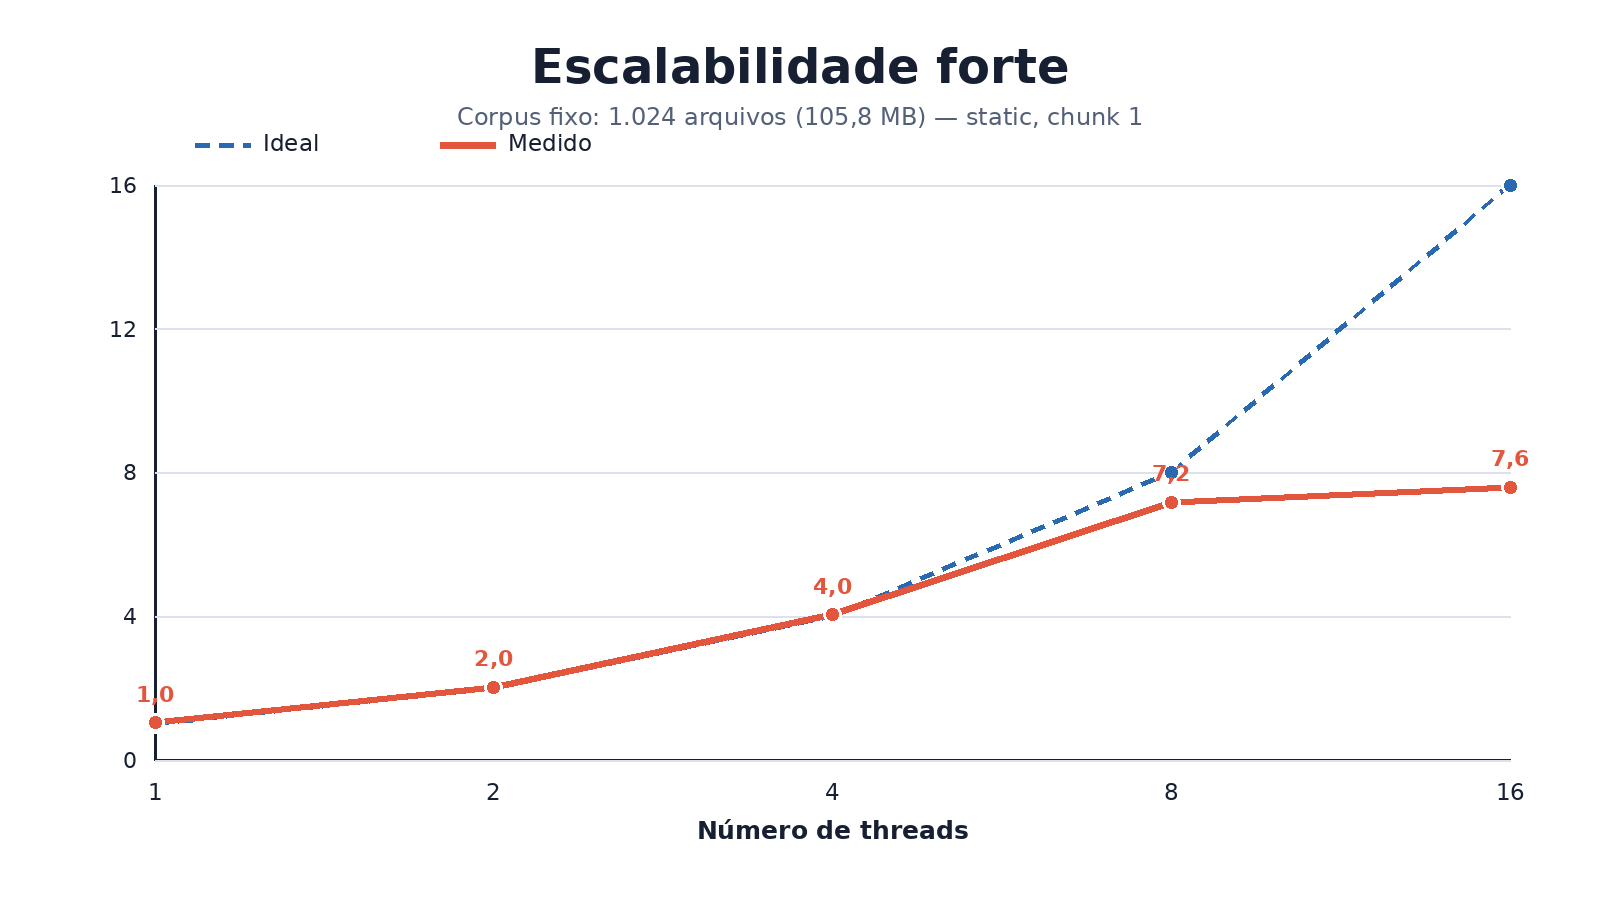
\includegraphics[width=\linewidth]{grafico_speedup_forte.png}
\end{minipage}\hfill
\begin{minipage}{0.48\textwidth}
  \centering
  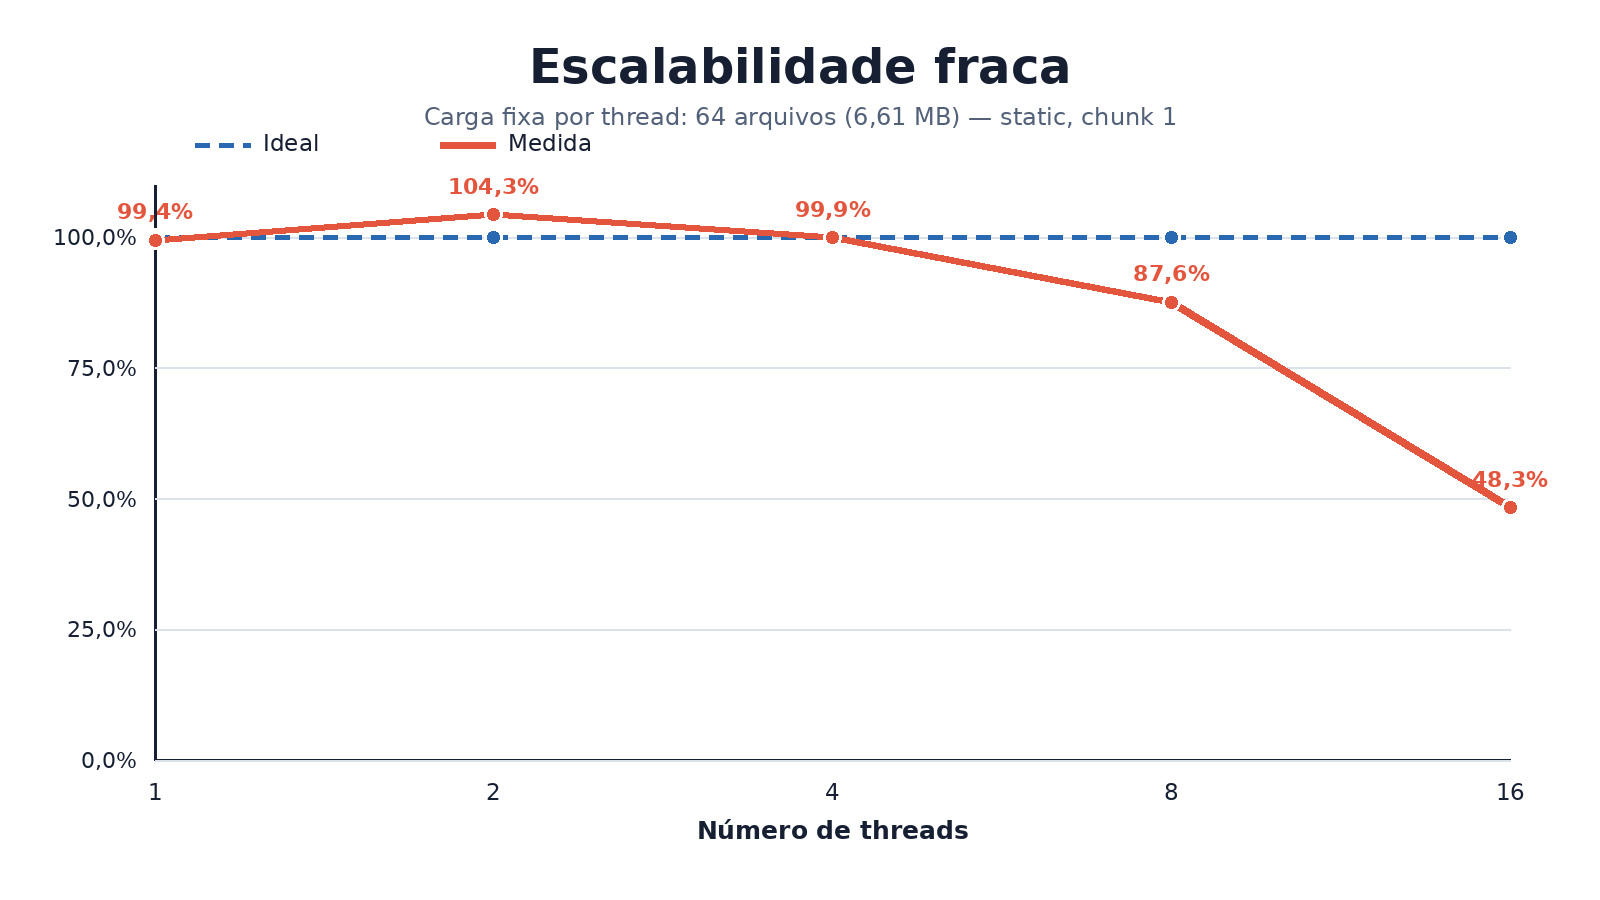
\includegraphics[width=\linewidth]{grafico_eficiencia_fraca.png}
\end{minipage}
\end{center}

\textbf{Melhor configuração observada por quantidade de threads}

\begin{center}
\begin{tabular}{rrrrr}
\toprule
Threads & Configuração & Tempo (ms) & Speed-up & Eficiência \\
\midrule
1  & \texttt{static,1}  & 209,847 & 1,033 & 103,3\% \\
2  & \texttt{dynamic,1} & 103,723 & 2,090 & 104,5\% \\
4  & \texttt{guided,1}  &  49,778 & 4,355 & 108,9\% \\
8  & \texttt{guided,4}  &  28,361 & 7,644 &  95,5\% \\
16 & \texttt{dynamic,1} &  26,545 & 8,167 &  51,0\% \\
\bottomrule
\end{tabular}
\end{center}

\clearpage
\section*{Código-fonte --- versão sequencial}
\lstinputlisting{buscador_sequencial.c}

\clearpage
\section*{Código-fonte --- versão paralela OpenMP}
\lstinputlisting{buscador_paralelo.c}

\end{document}
